\chapter*{Introduction}\label{chap:intro}\setcounter{page}{1}\frontmatter
\addcontentsline{toc}{chapter}{Introduction}
\chaptermark{Introduction}

When answering the classic question ``What is your Ph.D. about?'' to family and friends, I always start with the ``Ctrl + F'' function in their favourite text editor or web browser. This quickly highlights one of the applications of the exact pattern-matching problem. If I feel especially ambitious in my explanations, I will attempt to give the intuition of the naive $\Oh(nm)$ algorithm. Picture a young child, aligning the string against every position of the text and comparing character by character because the child has yet to learn how to read. To show a glimpse of a more complex solution, I comment on how, depending on the pattern, the child may try to skip portions of the text. But even my grandparents immediately know that efficient search in a text has been possible for decades and that it cannot be my real research subject.

\section{Context}

The exact pattern matching problem has been extensively studied, with in particular the famous Knuth-Morris-Pratt algorithm\footnote{The elegance of this algorithm is what first drew me in this area of research as a bachelor student!} published in 1977~\cite{KMP} after being independently discovered by Morris-Pratt in a technical report in 1970 and Knuth in 1973. Since then, this has become one of the classic textbook algorithms, and Charras and Lecroq published a detailed handbook~\cite{charras2004handbook} on the various solutions to exact pattern matching which have also been thoroughly compared in practice~\cite{DBLP:journals/corr/abs-1012-2547, faro2013exact}.


% String notations
In order to present the context of this thesis, we start with a few basic definitions. We assume the reader to be familiar with the little $o$, big $\Oh$, $\Omega$ , and $\Theta$ notations for complexities. %For lower bounds, we use the notation $f(n)=\Omega(g(n))$ to denote that $f$ is bounded bellow asymptotically by $g$. 
For ease of readability, we additionally use the notation $\Ohtilde$ that hides polylogarithmic factors. 
A string of length $n$ is a sequence $T[0] \dots T[n-1]$ of characters from a finite alphabet $\Sigma$ of size $\sigma$. The substring\footnote{I chose not to unify notations between publication so the substrings $T[i..j]$ is denoted $T[i...j]$  in Chapter~\ref{chap:gapped_index} and~\ref{chap:gapped_pm} and by $T[i,j]$ in Chapter~\ref{chap:LCS}.} $T[i..j]$ is the string $T[i] \cdots T[j]$.
%If $i > j$, then $T[i..j]$ is the empty string. 
We also use the notation $T[i..j)$ and $T(i..j]$ which stand for $T[i..j-1]$ and $T[i+1..j]$, respectively. We call the substrings of the form $T[0..i]$ \emph{prefixes}  and use the notation $T[..i]$, analogously \emph{suffixes} refer to substrings $T[j..n-1]$ and are denoted $T[j..]$. Given two strings $P$ and $T$, we say that $P$ occurs in $T$ at position $i$ if $i+|P| \leq |T|$ and $P=T[i..i+|P|-1]$.

% Complexities in algorithms vs DT 
Throughout this thesis, we assume the standard unit-cost word RAM model with words of size $\theta(N)$ for an input of size $N$. In this introduction, \emph{data structures} are seen as algorithms where the complexity analysis is split in two parts: the \emph{construction} and the \emph{query}. The construction is generally more expensive and meant to be performed once, whereas the queries are meant to be fast and performed multiple times with varying inputs, thus the focus is often on improving the space and time needed for the queries. 
%We also consider the streaming model that has a different complexity paradigm which we will present later on.


\subsection{Matching Models}\label{sec:intro:complex}

% Define center type column
\newcolumntype{Y}{>{\centering\arraybackslash}X}
\newcolumntype{P}[1]{>{\centering\arraybackslash}m{#1}}
\renewcommand\tabularxcolumn[1]{m{#1}}

%spacing
\renewcommand{\arraystretch}{2}
\begin{figure}[h]
    \begin{tabularx}{\textwidth}{P{3cm} P{4.5cm}  Y }
        Matching model & Pattern & Text with occurences underlined \\
        \hline
        Regular Expression~\cite{RM-704} & $P=$ GAT$(\mathrm{TA}\mid \mathrm{O})(\mathrm{CAT})^*$ & $T=$ \underline{GATTA}AT\underline{GATOCATCATCATCAT}A \\
        Error bound~\cite{landau1986efficient} (for ED~\cite{levenshtein1966binary}) & $P=$ GATTACAT & $T=$ AT\underline{GATTAACAT}ATA, $\mathrm{ED}(P,T[2..10])=1$ \\
        Don't care~\cite{fischer1974string} & $P=$ GAT**CAT & \underline{GATTACAT}A\underline{GATOACAT}AC\\
        %
        Gapped consecutive~\cite{bille2022gapped} & $P_1=$ GATTA $P_2=$ TAC  $a=2$, $b=6$ & $T=$ AGG\underline{GATTAC}TAC, $d=3 \in [a,b]$\\
        %
        Elastic Degenerate~\cite{iliopoulos2021efficient}  & $P=$ GATTACAT &  $T=$ {\renewcommand{\arraystretch}{1} AT\underline{GAT}$\left\{
            \begin{array}{l}
                \mathrm{\underline{TA}}  \\
                \mathrm{O}
            \end{array}\right\} \mathrm{\underline{CAT}A}$} \\
        %
        Abelian/Jumbled~\cite{eres2004permutation} & $P=$ GATTACAT & $T=$ AGAG\underline{TATGATC}AGT\\
        %
        Order preserving & $P =$ 1 5 3 4 6 2 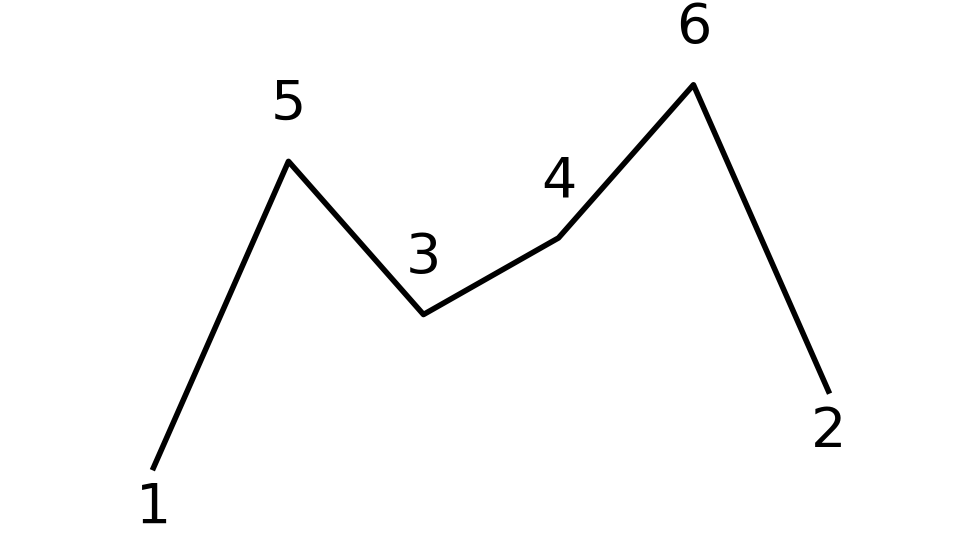
\includegraphics[width=3.5cm]{Introduction/op_P.png} & $T=$ \underline{2 7 4 5 8 3} \underline{1 20 15 16 25 6}  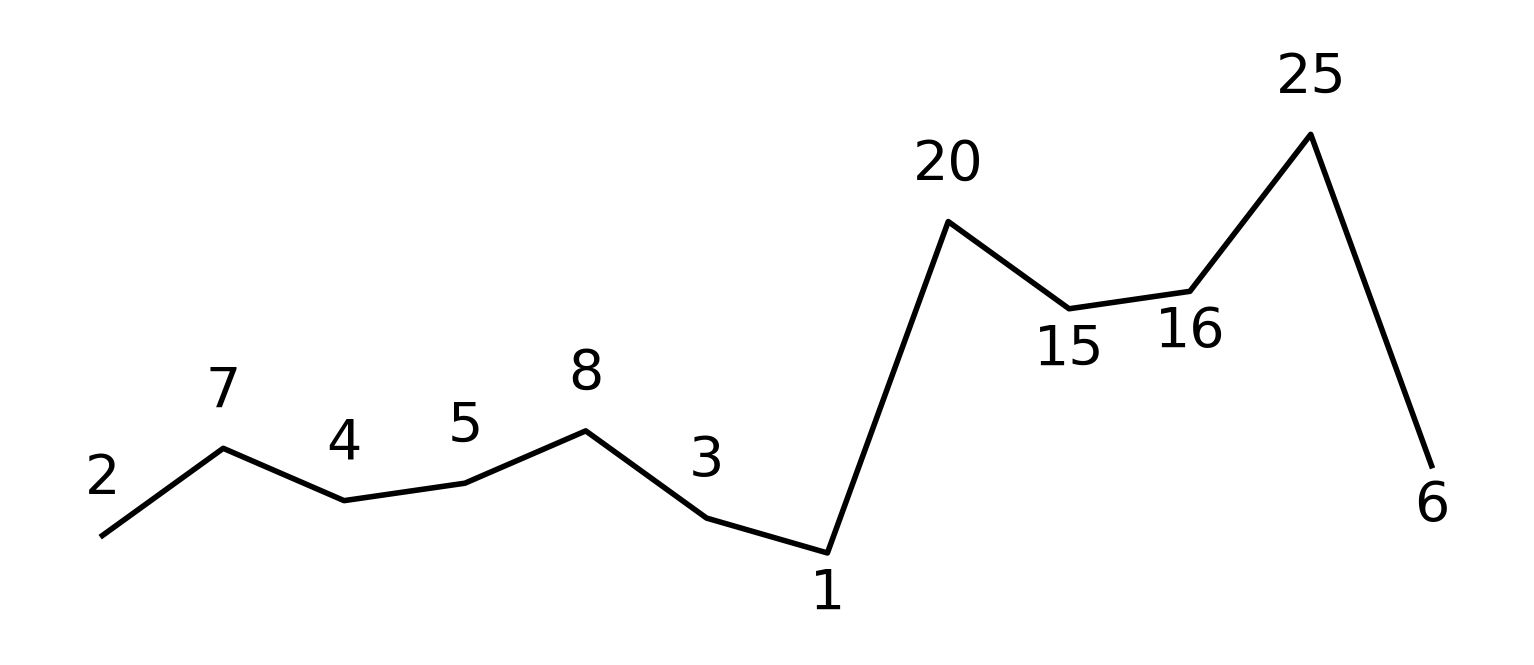
\includegraphics[width=5cm]{Introduction/op_T.png} \\
        %
        Parametrized~\cite{baker1993theory} & $P=$ GATTACAT & $T=$ OPO\underline{POGGODOG}O, {\footnotesize A:O, C:D, G:P, T:G} \\
    \end{tabularx}
    \caption{Example of various model of matching on strings.}
    \label{fig:intro:match_model}
\end{figure}

In general though, the need for text processing goes far beyond exact matching of patterns. To illustrate this claim, we present alternative models of matching with their motivations and specify those we study in the following chapters. Figure~\ref{fig:intro:match_model} also provides an example for each matching model.

% Regular expression
One of the oldest and most classic models for complex queries is \ul{regular expressions} search, introduced by Kleene in 1951~\cite{RM-704}.
% Explain the formalism
The regular expression formalism offers a concise description for sets of strings through recursive combinations of characters from an alphabet $\Sigma$ along with three fundamental operators: concatenation ($\cdot$), union ($|$), and Kleene star ($\ast$).
For two regular expressions $R_1$ and $R_2$ the concatenation $R_1\cdot R_2$ matches any concatenation of a string matching $R_1$ and a string matching $R_2$, the union $(R_1|R_2)$ allows matching any string matching either $R_1$ or $R_2$, and $(R_1)^\ast$ matches any number of repetitions of a string matching $R_1$, including no repetition, i.e. the empty string.
% Application
The use of regular expression gained popularity in the 1970s through their efficient implementation in Unix tools such as \texttt{awk}, \texttt{grep}, or \texttt{sed}.
They have become a crucial tool in many fields such as internet traffic analysis~\cite{4221791,4579527}, databases, data mining~\cite{1000341,10.5555/645927.672035,10.1145/375551.375569}, computer networks~\cite{10.1145/1159913.1159952}, and protein search~\cite{10.1145/369133.369220}.
% automaton
Another way to describe regular expressions is through the Thompson automaton construction~\cite{Thompson_automaton}. This automaton can then be simulated efficiently to test whether a string $T$ is recognized by a regular expression $R$ in $\Oh(|R| \times |T|)$ time.
% Lowerbounds
A series of works~\cite{10.1145/128749.128755,BILLE2008486,10.1007/978-3-642-02927-1_16,10.1007/11786986_56,doi:10.1137/1.9781611973075.104} has focused on improving the time complexity of regular expression search. However, they only managed to shave off polylogarithmic factors from the $\Oh(|R| \times |T|)$ complexity, and a recent fine-grained complexity approach brought an explanation for this.
Backurs and Indyk~\cite{DBLP:conf/focs/BackursI16} followed by Bringmann, Gr{\o}nlund, and Larsen~\cite{8104068} considered a subclass of regular expressions called ``homogeneous''. A regular expression is ``homogeneous'' if, in the tree representation of the expression, the operators at the same level are equal. For example $R=(P_1|P_2|...|P_d)^\ast$ is homogeneous and searching it corresponds to the Word break problem~\cite{wordbreak1,wordbreak2}. The authors of~\cite{DBLP:conf/focs/BackursI16,8104068} showed that every homogeneous regular expression search either allows for a solution in near-linear time or requires $\Omega((|R| \times |T|)^{1-o(1)})$ time conditioned on the Strong Exponential Time Hypothesis~\cite{IMPAGLIAZZO2001367}. The only exception is the Word break problem which can be solved in $\Oh(|T| (|R| \log |R|)^{1/3}+|R|)$-time has a matching lower bound up to polylogarithmic factors. Abboud and Bringmann~\cite{DBLP:conf/icalp/AbboudB18} further detailed those lower bounds using an even finer-grained complexity approach.
% Our work
These results give a good understanding of the time complexity of regular expression in the classical setting, however, multiple practical applications need to work with a stream of input. We specify what we mean by a stream later on in this introduction. Therefore, in Chapter~\ref{chap:regexp}, we provide a new space-efficient streaming algorithm for regular expression membership and pattern matching.


% Don't care
Although the versatility of regular expressions makes them widely used in practice across fields, they are notoriously difficult to write for users.
As a simpler alternative, Fischer and Paterson~\cite{fischer1974string} introduced the \underline{``don't care''} pattern matching where a don't care (also called wildcard or gap) symbol, denoted \texttt{?}, can occur in both the pattern and the text, and matches any other character of the alphabet.
% Space seed
This model has been directly applied in the PROSITE~\cite{hulo2006prosite} database of proteins where wildcards are supported. More generally, space seeds~\cite{li2004patternhunter}, a similar concept where only some positions have to be matched, have been used in homology search~\cite{ma2002patternhunter}, alignment~\cite{david2011shrimp2}, assembly~\cite{birol2015spaced}, and metagenomics~\cite{bvrinda2015spaced}.
% Gapped matching
Patterns with don't cares are sometimes~\cite{lewenstein2011indexing} described as $P= P_1g_1P_2g_2 \dots g_\ell P_{\ell+1}$ where $P_1$,$P_2$,\dots,$P_{\ell+1}$ are patterns over the alphabet $\Sigma$ and $g_1,g_2,\dots,g_{\ell}$ are the length of the maximal stretches of \texttt{?}. 
% variable length gap
Naturally this question was later extended to the problem of string matching with \underline{variable length gap}~\cite{bille2012string,bille2014string} where the length of the gaps can vary in intervals $[a_i,b_i]$ for $i\in[1,\ell]$.
% Applications
Note that variable length gaps are also supported by the PROSITE~\cite{hulo2006prosite} database.
% variants
Different variants of the problem have been studied~\cite{kopelowitz2016color,cohen2009range,brodal1999finding}, including a simpler version with just two patterns $P_1$ and $P_2$ and a single gap~\cite{peterlongo2006gapped,iliopoulos2009indexing} and the special case $P_1=P_2$~\cite{muthukrishnan2002efficient,keller2007range}.

% consecutive
In 2016, Navarro and Thankatchan~\cite{NAVARRO2016108} proposed a natural variant to pattern matching with a variable length gap, where given a single pattern $P$ and an interval $[a,b]$, one must report all consecutive occurrences of $P$ starting at positions $(i,j)$ (consecutive meaning no other occurrence in between $i$ and $j$) such that $j-i$ belongs to $[a,b]$. Since, consecutive occurrences have been studied in several publications~\cite{DBLP:conf/fsttcs/BilleGPRS20,cpm/BilleGPS21,DBLP:journals/corr/abs-2304-00887,DBLP:journals/corr/abs-2211-16860}.
% Gapped consecutive matching
Recently Bille et al.~\cite{bille2022gapped} proposed a combination of the gapped and consecutive lines of research: \underline{gapped consecutive matching} where we are given two patterns $P_1$ and $P_2$ as well as an interval $[a,b]$ and must report all consecutive occurrences of $P_1$ and $P_2$ with distance in $[a,b]$.
% Motivations
%This model can be linked to gapped q-grams~\cite{burkhardt2003better} which is an alternative to spaced seeds which were mentioned earlier.
% This thesis
We study gapped consecutive pattern matching in various settings in Chapters~\ref{chap:gapped_index} and~\ref{chap:gapped_pm}, a summary of the contribution is given in Section~\ref{intro:sec:contrib}.
%~\ref{chap:gapped_stream},

Although an in-depth non-standard matching listing is out of scope for this manuscript, for completeness, we detail other models found in the literature, and Table~\ref{fig:intro:match_model} provides examples for each of the models.
% Degenerate strings
The modelling of flexible and diverse DNA sequences~\cite{comm1970iupac} lead to the model of \underline{degenerate} strings~\cite{abrahamson1987generalized} (also called indeterminate), where each position corresponds to a subset of $\Sigma$. For bioinformatic applications, degenerate strings are most often used as pattern to search for (unlike the example I give in Table~\ref{fig:intro:match_model} where the text is degenerate but not the pattern).
% (Elastic/Generalised) Degenerate strings
This model has recently been extended in two directions: \underline{elastic degenerate} strings~\cite{iliopoulos2021efficient} where each position is a subset of strings over $\Sigma$ and \underline{generalized degenerate} strings~\cite{alzamel_et_al:LIPIcs:2018:9323} where each position is a subset of strings of $\Sigma^k$, and the length $k$ can vary from position to position.
% Weighted string
Alternatively, when each position is assigned a random variable with values in $\Sigma$ the strings are called \underline{weighted} (or uncertain) and represented by a weight matrix~\cite{thompson1994clustal}, see Table~\ref{fig:intro:match_model} for an example. Then, the cumulative probability that a string occurs at a starting position is the product of the probabilities of the corresponding characters at each position, and a match is often defined by a threshold on that cumulative probability. This model has been used in molecular biology in ``profiles'' that represent multiple aligned strings~\cite{doi:10.1073/pnas.84.13.4355} though they study a slightly different score: $\log \frac{p(x,i)}{p(x)}$ where $p(x,i)$ is the probability that the $i$th character is equal to $x$ and $p(x)$ is the overall frequency of $x$. 
% Abelian/jumbled/many other names 
In the model of \underline{Abelian} matching, a string (or a substring) is entirely identified by the characters it contains (with multiplicities), disregarding their order. It stems from the automatic discovery of clusters of genes in genomes where they can occur in a different order but still linked to the same function~\cite{eres2004permutation}, but the same concept has also been used in the context  of using mass spectrometry for DNA assembly~\cite{bocker2003sequencing} where the strings without order are called compomers. This model is also known as jumbled and permutation pattern matching, and several other names, see~\cite{ejaz2010abelian}.
% order preserving
The \underline{order-preserving} model~\cite{kim2014order,kubica2013linear} takes a somewhat opposite approach and says that two strings over an integer alphabet match if they have the same relative shape: $\forall i,j \in [0,n-1], X[i] < X[j] \leftrightarrow Y[i] < Y[j]$. This matching model aims at capturing the trend detection needed in the stock market and music melody matching problems~\cite{kim2014order}.
%
% Parametrized matching
Another application-driven model is \underline{parametrized strings} or ``p-string'' introduced by Baker~\cite{baker1993theory}, where two strings match if we can transform one into the other by applying a function renaming the parameters, meant to detect code duplication.


\subsection{Similarity Measures and Distances}
% The notion of robustness of the similarity measure
% Similarity measures
Many string applications have to work around noise in the input data, which makes it difficult to search for exact matches. Some of the models presented earlier define their match to take into account noisy input, but another important approach is to work with distances and similarity measures. Quantifying the degree of similarity and dissimilarity of two strings is for example needed in Bioinformatics~\cite{Gusfield1997}, music analysis~\cite{mongeau1990comparison}, and plagiarism detection~\cite{lukashenko2007computer}. 
%
A distance measure quantifies the dissimilarity between strings, while a similarity measure quantifies the degree of resemblance between strings. Most distances can be derived into similarity measure, and most similarity measure have a corresponding distance, thus in this section, we alternate between the two terms depending on which form is most common in the literature.

% Robustness to noise
Various types of noise can appear in the input, examples include single characters or entire words being replaced, inserted, or deleted, or some sections of the text being stretched or reordered. As a consequence, various similarity measures can be defined to account for the different types of noise, as the goal is always that a few noisy modifications do not modify drastically the distance to other strings.
% Hamming
One of the simplest distances on strings is the \underline{Hamming distance}: For two strings $X$ and $Y$ with $|X|=|Y|$, it is the number of mismatches between $X$ and $Y$. Alternatively, the Hamming distance is defined as the number of substitutions needed to transform $X$ into $Y$.
% Longuest Common Subsequence
When instead the goal is to have a similarity measure robust to insertions and deletions in the strings $X$ and $Y$, one can consider the length of the \underline{Longest Common Subsequence} between $X$ and $Y$: the largest $\ell$ such that there exist positions $i_1<... < i_\ell$ and $j_1< ... < j_\ell$ such that $X[i_p] = Y[j_p]$ for all $p \in [1,\ell]$. Note that the longest common subsequence has been used as the basis of comparison programs like \texttt{diff} which are then applied in version control systems like git.
% ED / Levenshtein
For the \underline{Levenshtein distance}~\cite{levenshtein1966binary} (also called the edit distance hereafter) the operations allowed are substitutions, insertions, and deletions, all with cost $1$. This definition can be generalized to allow costs to differ for each of the operations (weighted edit distance) or even for the cost to depend on which character is being added, removed or substituted (alphabet-weighted edit distance). This metric is one of the most well known, due to the importance of finding global alignments (alignments of two full strings with substitutions, insertions, and deletions) in bioinformatics~\cite{Gusfield1997}.
Unfortunately, Backurs and Indyk~\cite{DBLP:conf/stoc/BackursI15} proved a conditional lower bound (based on SETH) which suggests it is unlikely to be computable in strongly subquadratic time.
% LCS with $k$ mismatches
As an attempt to circumvent this lower bound, in Chapter~\ref{chap:LCS} we consider the \underline{Longest Common Substring (LCS) with Approximately $k$ Mismatches} an approximate version of a measure resilient to substitutions: \underline{LCS with $k$ Mismatches}. In the \kLCS problem, given an integer $k$ and two strings $X$ and $Y$, $\lcsk(X,Y)$ is the maximal length of a substring (must be continuous, unlike a subsequence) of $X$ that occurs in $Y$ with at most $k$ mismatches. 
But again, Kociumaka, Radoszewski, and Starikovskaya~\cite{DBLP:journals/algorithmica/KociumakaRS19} showed (conditioned on SETH) that there is $k=\Theta(\log n)$ such that \kLCS cannot be solved in strongly subquadratic time, thus they introduced \kApproxLCS with the goal of making the problem easier through approximation.
In Chapter~\ref{chap:LCS} we study that problem, where we are given a constant $\eps > 0$, and we need to return a substring of $X$ of length at least $\lcsk(X,Y)$ that occurs in $Y$ with at most $(1+\eps) \cdot k$ mismatches. We provide two new algorithms with different space-time trade-offs and evaluate the speed of one of them in practice compared to the quadratic dynamic programming solution for \kLCS. In Section~\ref{intro:sec:contrib}, we further detail our contributions.
%\todo[inline]{Replace the last sentence by a more concrete and concise description of my contrib.}

% Approximate matching
Apart from the direct comparison of two strings, distances are also used to define approximate matching problems~\cite{landau1986efficient,landau1989fast} where for a given integer $\tau$, a pattern $P$, and a text $T$, one must report all positions $j$ such that there is a substring $T[i..j]$ that is at distance at most $\tau$ from $P$.
For a survey on the results before 2001 on approximate matching for the Edit, Hamming and Longest Common Subsequence distances, see~\cite{navarro2001guided}.
% DTW
We study approximate matching in Chapter~\ref{chap:DTW} with regard to a popular distance for temporal sequences, which is less common for strings: the \underline{Dynamic Time Warping (DTW) distance}~\cite{sakoe1978dynamic}. For strings, the DTW distance can be described as follows: duplicate some characters to obtain strings of equal length and to minimize the sum of the distances between the characters at the same positions, this sum is the DTW distance. Computing the edit distance (for a given metric space over the characters) has been reduced to computing DTW~\cite{DBLP:conf/icalp/Kuszmaul19} (over the same metric space, just with an added null character).
%
All similarity measures and distances mentioned above are illustrated in Figure~\ref{fig:intro:similarities}.
% PM


\newcolumntype{E}[1]{>{\small \arraybackslash}m{#1}}
\newcolumntype{R}{>{\raggedleft\arraybackslash}X}

\begin{table}
    \small
    {\renewcommand{\arraystretch}{1.5}
    \begin{tabularx}{\textwidth}{E{10cm}   R}
        Similarity measure & Example~~~ \\
        \hline\\
        % Hamming
        \begin{minipage}{10cm} \renewcommand{\arraystretch}{1}
        Hamming distance  \\
        $$\mathrm{HD}(X,Y)=  \left\{
            \begin{array}{l}
                +\infty \mbox{ if } |X| \neq |Y| \mathrm{,}\\
                |\{ i \mbox{ s.t. } X[i]\neq Y[j] \}| \mbox{, else.}
            \end{array} \right.$$
        \end{minipage}
        &
        \hfill
        \begin{minipage}{4cm} \renewcommand{\arraystretch}{1}
            \hfill
            $\begin{array}{r}
                X= \mathrm{\texttt{AAAATG}}\\
                \mathrm{ \texttt{|||**|}}\\
                Y= \mathrm{\texttt{AAATCG}}\\
                \mathrm{HD}(X,Y)=2
            \end{array}$
            \vspace{0.4cm}
        \end{minipage}\\
        %
        \arrayrulecolor{gray}\hline \\
        % LCSubsequence
        \begin{minipage}{10cm} \renewcommand{\arraystretch}{1}
        Length of the Longest Common Subsequence \\
        $$ \mathrm{LCSeq}(X_i,Y_j)= \left\{
            \begin{array}{l}
                0 \mbox{ if } i=0 \mbox{ or } j=0 {,}\\
                \mathrm{LCSeq}(X_{i-1},Y_{j-1})+1 \mbox{ if } X[i]=Y[j]\mbox{,} \\
                \max(\mathrm{LCSeq}(X_{i-1},Y_j),\mathrm{LCSeq}(X_i,Y_{j-1})) \mbox{, else.}
            \end{array} \right. $$
            \vspace{0.4cm}
        \end{minipage}
        &
        \hfill
        \begin{minipage}{4cm} \renewcommand{\arraystretch}{1}
            \hfill
            $\begin{array}{r}
                X= \mathrm{\texttt{AAAAGC}}\\
                Y= \mathrm{\texttt{\underline{AA}T\underline{C}}}\\
                \mathrm{LCseq}(X,Y)=3
            \end{array}$
        \end{minipage}\\
        \arrayrulecolor{gray}\hline \\
        % ED
        \begin{minipage}{10cm} \renewcommand{\arraystretch}{1}
            Levenshtein/Edit distance \\
            $$ \mathrm{ED}(X_i,Y_j)= \left\{
                \begin{array}{l}
                    \max(i,j) \mbox{ if } i=0 \mbox{ or } j=0 {,} \\
                    \mbox{else, } \min 
                    \begin{pmatrix}
                        \mathrm{ED}(X_{i-1},Y_{j-1})+d(X[i],Y[j]), \\
                        \mathrm{ED}(X_{i-1},Y_j)+1, \\
                        \mathrm{ED}(X_i,Y_{j-1})+1
                    \end{pmatrix} 
                \end{array} \right. $$
                \vspace{0.4cm}
            \end{minipage}
            &
            \hfill
            \begin{minipage}{4cm} \renewcommand{\arraystretch}{1}
                \hfill
                $\begin{array}{r}
                    X= \mathrm{\texttt{AAAATG}}\\
                    \mathrm{\texttt{||~~|*}}\\
                    Y= \mathrm{\texttt{AA-{-}TC}}\\
                    \mathrm{ED}(X,Y)=3
                \end{array}$
        \end{minipage}\\
        \arrayrulecolor{gray}\hline \\
        % DTW
        \begin{minipage}{10cm} \renewcommand{\arraystretch}{1}
            \textbf{Dynamic Time Warping distance} \\ 
            $$ \mathrm{DTW}(X_i,Y_j)= \left\{
            \begin{array}{l}
                0 \mbox{ if } i=0 \mbox{ and } j=0 {,} \\
                +\infty \mbox{ else if } i=0 \mbox{ or } j=0 {,} \\
                \mbox{else, } \min 
                \begin{pmatrix}
                    \mathrm{DTW}(X_{i-1},Y_{j-1}), \\
                    \mathrm{DTW}(X_{i-1},Y_j), \\
                    \mathrm{DTW}(X_i,Y_{j-1})
                \end{pmatrix} + d(X[i],Y[j])
            \end{array} \right. $$
            \vspace{0.4cm}
        \end{minipage}
        &
        \hfill
        \begin{minipage}{4cm} \renewcommand{\arraystretch}{1}
            \hfill
        $\begin{array}{r}
            X= \underbrace{\mathrm{\texttt{AAAA}}}\mathrm{\texttt{TG}}\\
                \mathrm{\texttt{~||~|*}}\\
            Y= \mathrm{\texttt{~AA~TC}}\\
            \mathrm{DTW}(X,Y)=1
        \end{array}$ 
    \end{minipage}\\
    \arrayrulecolor{gray}\hline \\
    % LCSubstring
    \begin{minipage}{10cm} \renewcommand{\arraystretch}{1}
        \small \mbox{Length of the Longest Common Substring} \\
        $$ \mathrm{LCS}(X,Y)= \max \{ l+1, \exists i,j \mbox{ s.t. } X[i:i+l]=Y[j:j+l] \}$$
        \end{minipage}
        &
        \hfill
        \begin{minipage}{4cm} \renewcommand{\arraystretch}{1}
            \hfill
        $\begin{array}{r}
            X= \mathrm{\texttt{AA\underline{AAT}G}}\\
            Y= \mathrm{\texttt{~\underline{AAT}TCG}}\\
            \mathrm{LCS}(X,Y)=3
        \end{array}$
        \vspace{0.4cm}
    \end{minipage}\\
    \arrayrulecolor{gray}\hline \\
    % LCSubsting with k mismatches
    \begin{minipage}{10cm} \renewcommand{\arraystretch}{1}
        \small \mbox{\textbf{Length of the Longest Common Substring with $k$ Mismatches}} \\
        $$ \lcsk(X,Y)= \max \{ l+1, \exists i,j \mbox{ s.t. } \mathrm{HD}(X[i:i+l],Y[j:j+l]) \leq k \}$$
        \end{minipage}
        &
        \hfill
        \begin{minipage}{4cm} \renewcommand{\arraystretch}{1}
            \hfill
        $\begin{array}{r}
            X= \mathrm{\texttt{A\underline{AAATG}}}\\
            Y= \mathrm{\texttt{~\underline{AATTC}G}}\\
            \mathrm{LCS}_2(X,Y)=5
        \end{array}$
    \end{minipage}\\
    \end{tabularx}
    }
    \caption{Example for various similarities, in bold those we study in this thesis, for a given metric $d:\Sigma \times \Sigma \rightarrow \mathbb{Z}^{+}$ over the alphabet. For two given strings $X$ and $Y$ and two integers $0 \leq i < |X|$ and $0 \leq j < |Y|$, for compactness, $X_i$ and $Y_j$ denote the prefixes of $X$ and $Y$ of length $i$ and $j$ respectively.}
    \label{fig:intro:similarities}
\end{table}
\renewcommand{\arraystretch}{1}

\subsection{Repetition Detection}

We discussed pattern matching models and similarity measures, we now move to another central task in string processing: repetition detection. Locating repeated fragments inside a string can be useful to detect duplicated data to be removed or to compress its representation. For example, decomposing a string into maximal fragment that appeared earlier (and appending the next symbol) is the basis of the Lempel--Ziv factorization~\cite{ziv1977universal}. Once detected, highly repetitive regions of a string can also be treated differently (see~\cite{Porat:09} for example) allowing for a more efficient algorithm overall.

In music~\cite{arom1989time}, genomic~\cite{pich2018somatic}, finance~\cite{harvey2007trends} and astronomy~\cite{hewish1979observation}\footnote{ When Jocelyn Bell first discovered signals coming from pulsars (a rotating neutron star that creates a lighthouse effect), their regularity was so surprising that speculations where made on the fact that they might be signal from extraterrestrial intelligence.}, a number of dataset present signs of repetition of a periodic phenomenon.
Formally, we say that a string $T$ of length $n$ is periodic with period $p \leq n/2$ if for all $0 \leq i < n - p$, $T[i]=T[i+p]$, and the smallest period of $T$ is simply called the period of $T$.
%
But often, input data only contains periodic substrings (rather than being entirely periodic), which naturally leads to the concept of runs. Runs are maximal substrings that are periodic with a given period, i.e. a substring $T[i..j]$ is a run if it is periodic with period $p$, and $T[i-1..j]$ and $T[i..j+1]$ (if well-defined, i.e. $0<i$ and $j<|T|-1$) are not periodic with period $p$. 

A simpler model often considered is squares: substrings $T[i..i+2k-1]$ such that $T[i..i+k-1]=T[i+k..i+2k-1]$, it is referred to as a square or a tandem. This form of repetition naturally occurs in DNA and plays an important role in genomic fingerprinting~\cite{Kolpakov2003,GYMREK20179}. 
%
The study of squares in strings goes back to 1906 with the work of Thue~\cite{thue1906} on the construction of an infinite square free word. In terms on algorithm, the most basic question is testing whether a string of length $n$ contains at least one square, and it was first considered by Main and Lorentz~\cite{Main1984} who design an $\Oh(n \log n)$ time algorithm. They used a divide and conquer approach that can be adapted to report a compact representation of all squares in the same time complexity. At the same time they showed that $\Omega(n\log n)$ comparisons (checking if two characters are equal) where necessary, but their proofs uses strings with up to $n$ distinct characters. Therefore, they left as an open question whether a faster algorithm could be designed when the alphabet size is restricted.  
And indeed, we show in Chapter~\ref{chap:squares} that for a string over an unordered alphabet of size $\sigma$, there is an algorithm for testing whether it contains a square in $\Oh(n\log \sigma)$ time using only equality tests to compare characters. We also show that this result is optimal for deterministic algorithms and we extend it to reporting all runs in the string.

Many other forms of string regularities have been considered in the literature. Although they are out of the scope of this thesis, we list a few of them for completeness.
% Palindromes
Palindromes are strings that are identical when read backward or forward, formally, a string $T$ of length $n$ is a palindrome if $T[n-1] \dots T[1]T[0] = T[0]T[1] \dots T[n-1]$. Palindromes are found in music~\cite{tablecannon,crabcannon} and genomes~\cite{brazda2016palindrome,svetec2021palindromes} where they are linked to the regulation of gene replication and implicated in the evolution and development of diseases such as cancer and neurodegenerative disorders.
% Covers
Another way to view repeated fragments is through the lenses of string covers~\cite{iliopoulos1996covering}. A string $C$ is a cover of a string $T$ if $T$ occurs in a string constructed by overlapping and concatenating occurrences of $C$. A substring of $T$ is called a seed if it covers $T$ and a cover of minimal length is called a quasiperiod of $T$. 
Those notions generalize the concept of periods in the sense that they additionally allow for superposition of the repetitions, but other approaches have been considered as generalizations.
% Cadences
Cadences~\cite{AMIR20174} in a string are characters that are repeated at regular intervals. Formally, given a string $T[0,n-1]$, a cadence is a pair $(i,d)$ such that $0 \leq i,d < n$ and for every $k \geq 0$ such that $i+kd < n$ we have $T[i] = T[i+kd]$. Intuitively, a cadence defines a periodicity that is woven regularly inside an aperiodic string.
% Approximate periodicity
Approximate periodicity has been considered as well. A series of publications~\cite{SIM2001557,AMIR2015215,AmirICALP2010, KociumakaRADO2018, AMIR20182} studied the problem of deciding whether a given string is close to any periodic string under a given metric.
% finding approximate periodic progressions
%Other works~\cite{AMIR201460,Gfeller2011} focus on approximate periodic progressions. They take as input a sequence of increasing integers and then define an approximate periodicity in the progression of numbers.

% Substring equations
Interestingly, a number of those definitions can be formulated through substring equations and Gawrychowski et al.~\cite{GAWRYCHOWSKI2020174} gave an algorithm that from a set of substring equations over strings of length $n$ can produce a ``generic'' solution which contains a maximal number of different characters and from which every solution can be generated through character renaming. They gave an algorithm producing a generic solution in $\Oh(n)$ which generalizes solutions to various reconstruction problems such as reconstructing a string from its maximal palindromes or runs.

\subsection{Scalability Issues}\label{sec:intro:scalability}

%%%%%%%%%%%%%%%%%%%%%% Intro scalibility %%%%%%%%%%%%%%%%%%%%%%%%%%%%
 
% But it is not just about the specific model also about scalibility
We discussed so far how string processing tasks have crucial industry-relevant applications, but another major challenge in most applications is the scalability to large datasets.
% Wikipedia
Highly curated datasets generally remain quite small. For example, the English pages of Wikipedia (just the text and metadata) take up 20~gigabytes in a compressed format as of 2022~\cite{wikimedia}. In comparison, any form of archival and version history tends to grow much bigger. Just the metadata of revision's history (without the content of the articles) for the Wikipedia English pages occupies 75~gigabytes as of 2022.
% Software Heritage
It is sometimes possible to limit the redundancy in the archival data, for example by using a graph which tracks where the data is repeated multiple times. This is the approach taken by the Software Heritage~\cite{swh-site} project, which aims at keeping an archive of entirety of the software code produced by humanity. The graph structure is especially necessary in this project to reduce code redundancy and reflect the standard use of version history management in software development.
Substantial research and engineering efforts~\cite{DBLP:phd/hal/Pietri21} were made to provide an efficient navigation of the graph. 
However, since the code repositories are indexed based on their URLs and metadata, it is not currently feasible to perform a search specifically for occurrences of a particular code snippet\footnote{\setlength\parindent{10pt} A simple but interesting example is~\cite{vii2014if} where the author searched \texttt{"const double epsilon ="} (and equivalents in other languages) on all GitHub repositories to study the value programmers typically chose for epsilon.}.
As of 2023, the graph is limited to 7~terabytes but with the source files the space usage approaches 1~petabyte~\cite{swh-polytechnique}.
% Internet archive
Another example of a large archival project is the internet archive, a non-profit which started saving web pages in 1996 and now holds the history of more than 800 billion web pages through their program: the wayback machine~\cite{web-archive}. This archive takes up more than 70~petabytes, and is still growing quickly (see Figure~\ref{fig:scalability}).
Here, again, the search options are limited to the metadata of the websites and not the content of the webpages themselves.


%%%%%%%%%% Bioinformatics
%Intro DNA representation
Large archives also exist in bioinformatics, but the structure of biological sequences is very different from that of code or webpages, which are typically structured, with links, a large alphabet, and a reasonable number of distinct words.
% DNA Introduction
The genetic information encoded in DNA can be abstracted as just a string over the nucleotide alphabet \texttt{\{A, T, C, G\}}.
We obtain this string after sequencing and assembling. When a genome is sequenced, the output is a set of fragments, called \emph{reads}, extracted from the original sequence. Reads can contain sequencing errors, including nucleotide insertions, deletions, and substitutions. The typical length and error rate of the reads vary depending on the sequencing techniques.
%
In any case, the original position of the read in the genome is lost during sequencing and the reads have to be aligned and merged in order to reconstruct the original genome, this problem is called sequence assembly. To make this reconstruction possible, the read are extracted in such quantities that each position of the original genome is covered multiple times. This makes readsets larger and more redundant than the assembled genome. 
An additional difficulty is that DNA is composed of two chains of complementary nucleotides (\texttt{A-T, C-G} pairing). During sequencing, those complementary chains are detached and processed in opposite directions, and reads come from both, thus, when assembling or aligning to a reference it is necessary to consider the reverse complement of a read.


% Redundancy
Bioinformatics applications work with sequences that are generally redundant either from repeated regions in a genome (intra-genome redundancy) or by considering several genomes (from the same species) that share portions of their genomes (inter-genome redundancy).
% Single sequence indexes 
Exploiting this redundancy is key to providing efficient algorithms, an example of that is the problem of indexing a single string.
If the DNA is stored just as a string over the nucleotide alphabet \texttt{\{A, T, C, G\}}, it uses just 2 bits per base but requires linearly scanning the whole string to search for a pattern. 
Alternatively, the suffix tree is a classical structure that enables more efficient sequence analysis but necessitates 10 bytes per base~\cite{navarro2016compact}, which amounts to 30 gigabytes for a human genome containing 3.3 billion bases. 
This would not be practical for projects where thousands of genomes have been sequenced such as the 1000 Genomes project~\cite{10002015global} completed in 2015 and the 100K Genomes project~\cite{100Kgenomes} completed in 2018. 
Fortunately, compact data structures that exploit redundancy to decrease space usage offer an interesting trade-off: for a human genome it allows representing the sequence and its suffix tree using just 4 gigabytes~\cite{navarro2016compact}.

% Cheaper = more sequencing
Scalable algorithms are crucial for bioinformatics as there has been a drastic decrease in sequencing cost and an increase in throughput since 2008 (faster than expected by Moore's law~\cite{muir2016real}) which both lead to higher volumes of DNA being sequenced. 
% ENA
So far, the European Nucleotide Archive has accumulated more than 50 petabytes~\cite{ena} of sequencing data.
% SRA
While the NCBI Sequence Read Archive has more than 73 petabases~\cite{sra} of data including 38 petabases in open access and is still growing, see Figure~\ref{fig:scalability}. However, like for the software heritage project and internet archive, in the ENA and the NCBI, the data is indexed solely based on its metadata.
% Link to this thesis 
In Chapter~\ref{chap:XBWT}, we propose a compact index specifically designed for sets of short reads, that takes advantage of the redundant input to achieve better compression and scalability. 


\begin{figure}
    \centering
    \begin{subfigure}[b]{0.45\textwidth}
        \begin{tikzpicture}
            \node (img) {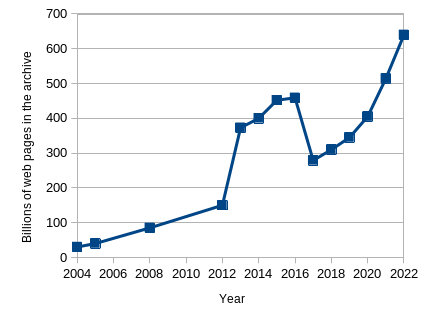
\includegraphics[width=0.95\textwidth]{0_sheets/wayback_machine.png}};
            \node [below right,text width=2.7cm,align=center, fill=white] at (0.25,-0.5){{\fontsize{7pt}{6pt}\selectfont Pages removed due to security concerns.}};
            \draw[->] (1,-0.5) -- (1.3,0.3);
        \end{tikzpicture}
        \caption{The Wayback Machine Archive}
    \end{subfigure}
    \begin{subfigure}[b]{0.49\textwidth}
    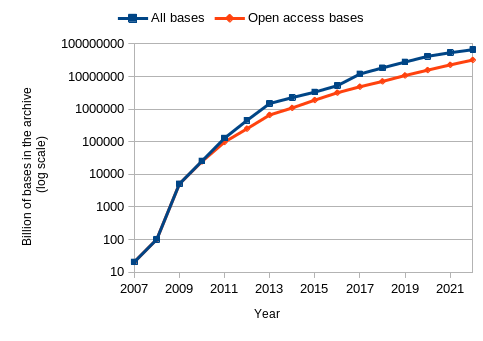
\includegraphics[width=\textwidth]{0_sheets/sra_growth.png}
    \caption{The Sequence Read Archive}
\end{subfigure}
\caption{Plots of the database growth for the Wayback Machine~\cite{web-archive-growth} and the Sequence Read Archive~\cite{sra}. The databases are big but also still quickly growing.}
\label{fig:scalability}
\end{figure}
